\chapter{Methods}

Considering the huge dimension of the dataset and the fact that a large portion of its content was
useless, smaller datasets have been computed with the aim of expediting the analysis even for future
usages. The analysis was made based on the computed datasets. 

\bigskip



\tikzstyle{square} = [rectangle, rounded corners, minimum width=3cm, minimum height=1cm,text centered,text width=3cm, draw=black, fill=blue!20]
\tikzstyle{arrow} = [thick,->,>=stealth]

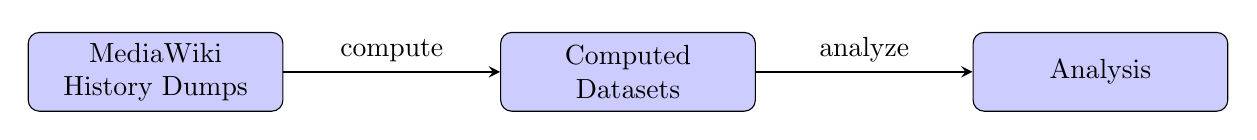
\begin{tikzpicture}[node distance=4cm]
    \node (dataset) [square, xshift=4cm] {MediaWiki History Dumps};
    \node (computed) [square, right of=dataset, xshift=2cm] {Computed Datasets};
    \node (anal) [square, right of=computed, xshift=2cm] {Analysis};

    \draw [arrow] (dataset) --node[anchor=south] {compute}(computed);
    \draw [arrow] (computed) -- node[anchor=south]{analyze}(anal);

\end{tikzpicture}

\bigskip

\section{Computed Dataset}
In the first skim only the revisions that were involved in a revert remained. This dataset, which
schema is the same as the MediaWiki History Dumps, has been ordered by page and thanks to this
screening, now the size of the dataset is ~10\% of the original. 

From this filtered dataset have been computed several smaller datasets which can be divided into 2 modules: 

\begin{itemize}
    \item Chains: in these datasets, the focus was on detecting revert chains in pages 
    \item Group: in these datasets, the focus was on the number of reverts that users did or received basing on the groups ( admin, registered, anonymous).
\end{itemize}

\subsection{Chains}
The data about revert chains were computed from the filtered dataset. The output is a JSON file, to
each page corresponds a JSON object. For each page is saved the list of chains and some statistics.
A chain has a start and an end date, a list of revisions, and the users involved. This dataset is
way smaller than the initial so it's possible to browse the dataset in few seconds.  
In the schema below there are all the fields in a page object. 

\begin{verbatim}
    {
        "title": "Loligo_vulgaris", 
        "chains": 
        [{
            "revisions": ["113715375", "113715381", "113715393"], 
            "users": {"62.18.117.244": "", "Leo0428": "17181"}, 
            "len": 3, 
            "start": "2020-06-15 22:16:23.0", 
            "end": "2020-06-15 22:17:38.0"
        }], 
        "n_chains": 1, 
        "n_reverts_in_chains": 3, 
        "n_reverts": 38
        "mean": 3.0, 
        "longest": 3, 
        "G": 0,
        "M": 0, 
        "lengths": {"3": 1}
    }
    
\end{verbatim}


With regard to users, the object is very similar and it is computed from the JSON of the page. The
only difference is that there is not the M field because it is only related to a page. G, instead,
can be computed on a user considering every chain where it is the author of at least a revision.

The data is also been computed monthly, the schema is simplier than the JSON one and this allow us
to save it in a TSV using only a row for each month. Instead of saving all the data about the chain
it is saved the number of chains which ar longer than 5,7,9.
\begin{table}[H]
    \centering
    \ra{1.2}
    \begin{tabularx}{\columnwidth}{@{}Xcccccccccc@{}}
        \midrule
        \textbf{title} & \textbf{year\_month} & \textbf{nchain} & \textbf{nrev} & \textbf{mean} & \textbf{longest} & \textbf{$\geq$ 5} & \textbf{$\geq$ 7} & \textbf{$\geq$ 9} & \textbf{G}\\ \toprule
        Loligo\_vulgaris & 2020-10 & 1 & 15 & 3.0 & 3 & 0 & 0 & 0 & 0\\
        
         \bottomrule
    \end{tabularx}
    
    \caption{entry of the mothly tsv \label{table:chainsPage}}
\end{table}


\subsection{Group}
Another interesting part of the study was focusing on the category a user belongs. Thanks to this we
are able to track the habits of the users allowing us to understand, for example, if someone stops
editing Wikipedia after several reverts from admins. Detecting these kinds of patterns is useful for
community health: a user can be warned if its behavior could lead to a drop-off. The groups to which
users can belong are: 
\begin{itemize}
    \item Admin (sysop): can perform certain actions like blocking users and editingprotected pages, 
    \item Registered: are logged in at the time of the edit, 
    \item Anonymous: are notlogged in and their username is their IP address(it is not possible to match an IP with a user
        because the IP can change over time).
\end{itemize}

The datasets computed are both for pages and users: 
\paragraph*{Pages} 
For each page, there are two topics of investigation: reverts and mutual reverts. An entry of the
dataset is a page-month and gives us the number of reverts and mutual reverts made on the page
divided by group. This can be helpful, for example, to detect pages where admins are more active and
this could be a sign that something is wrong with the page.



The notation \textit{adm\_reg} in table \ref{table:revertpage} refers to the number of admin that performed a
revert to a registered user (similarly with \textit{adm\_adm, reg\_adm, reg\_reg} ).\\

The notation \textit{mut\_ra} in the table \ref{table:mutualpage} refers to the number of mutual reverts
where the users involved are a registered one and an admin, the order does not matter, in fact, there is
no \textit{mut\_ar} that would have the same value.\\


Since the focus was on experienced users only pairs involving registered and admins were calculated.
For having an idea of the volume of the reverts made by anon it's been saved the number of reverts
that were made by anonymous (\textit{anon}) and not (\textit{not\_anon}).
\begin{table}[H]
    \centering
    \ra{1.2}
    \begin{tabularx}{\columnwidth}{@{}Xcccccccccc@{}}
        \midrule
        \textbf{id} & \textbf{page} & \textbf{year\_month} & \textbf{adm\_adm} & \textbf{adm\_reg} & \textbf{reg\_adm} & \textbf{reg\_reg} & \textbf{anon} & \textbf{not\_anon}\\ \toprule
        1 & pagina & 2020-10 & 13 & 12 & 42 & 0 & 0 & 0 \\
        
         \bottomrule
    \end{tabularx}
    
    \caption{entry of the revert page tsv \label{table:revertpage}}
\end{table}

\begin{table}[H]
    \centering
    \ra{1.2}
    \begin{tabularx}{\columnwidth}{@{}Xcccccccccc@{}}
        \midrule
        \textbf{id} & \textbf{page} & \textbf{year\_month} & \textbf{mut\_aa} & \textbf{mut\_ra}  & \textbf{mut\_rr} & \textbf{anon} & \textbf{not\_anon}\\ \toprule
        1 & pagina & 2020-10 & 13 & 12 & 42  & 0 & 0 \\
         \bottomrule
    \end{tabularx}
    
    \caption{entry of the mutual page TSV \label{table:mutualpage}}
\end{table}

\paragraph*{User}
It's useful also to have the data aggregated by user. The data for the reverts can be retrieved from
the filtered dataset sorted by timestamp. The data about reverts is gathered and processed month by
month, this allowed us to save for each user-month the number of reverts made and received divided by group.


\begin{table}[H]
    \centering
    \ra{1.2}
    \begin{tabularx}{\columnwidth}{@{}ccc@{}}
        \midrule
        \textbf{user} & \textbf{group} & \textbf{year\_month} \\ \toprule
        carlos & adm & 2020-10  \\
        
         \bottomrule
    \end{tabularx}
    \begin{tabularx}{\columnwidth}{@{}XXXXXXXX@{}}
        \midrule
        \textbf{received} & \textbf{r\_reg}  & \textbf{r\_not} & \textbf{r\_adm} & \textbf{done} & \textbf{d\_reg} & \textbf{d\_not} & \textbf{d\_adm}\\ \toprule
        13 & 12 & 42  & 0 & 13 & 12 & 42  & 0  \\
        
         \bottomrule
    \end{tabularx}
    
    \caption{entry of the mutual page tsv \label{table:revks}}
\end{table}


The mutual revert one was harder to achieve because for saving the information about mutual reverts
we need the dataset sorted by pages, but for having the data by user we should use the one sorted
by timestamp. We solved this problem by saving in the dataset the user-page-month, so the information
about mutual reverts a user performed in a specific month in a specific page. This led to a larger dataset but with a
higher level of information: it is easy to post-process the dataset by grouping by user or by month
to have one entry per user or one entry per month, respectively. 


\begin{table}[H]
    \centering
    \ra{1.2}
    \begin{tabularx}{\columnwidth}{@{}XXXXXXX@{}}
        \midrule
        \textbf{user} & \textbf{group} & \textbf{page\_name}& \textbf{year\_month} & \textbf{mut\_adm}& \textbf{mut\_reg}& \textbf{mut\_not}\\ \toprule
        khalu & adm & pagina & 2020-10 & 13 & 12 & 4 \\
        
         \bottomrule
    \end{tabularx}

    
    \caption{entry of the mutual page tsv \label{table:rjevks}}
\end{table}




\section{Analysis}
The second step of this work was the analysis of the dataset just generated. Thanks to the structure
and the heavy pruning analyzing these datasets is fast, This allows us to have a better workflow
without interruptions. We analyzed the data in 2 ways: a descriptive statistic and an interactive
one.
\paragraph{Descriptive}
For each dataset there is a script that runs and plots various statistics using the python libraries
Pandas and Matplotlib. There are 2 types of output: plots and rankings. 
Plots are useful to understand the trend from a more comprehensive point of view month by month.  
Rankings instead are used to see in a more specific way the pages/users ordered by one of the
metrics previously computed 

\paragraph{Interactive}
The other group members and I decided to make available online an interactive dashboard. The idea is
that everyone can change a few parameters and see how the metrics are performing in a personalized
way. To achieve this we uploaded our dataset on a database and thanks to an innovative way to retrieve
data (grapQL) we can display it on a website.

